\documentclass[11pt]{article}

% ===========================================================================
% PLAIN-LANGUAGE COMPANION (placeholder)
% A non-mathematical rendition of the framework in main.tex, for water
% managers, program staff, and attorneys. It sits between the peer-reviewed
% paper and the guidance for the Conserved Water Ledger tool.
% Candidate venues: The Water Report; Journal of Contemporary Water Research
% & Education (JCWRE, UCOWR). Format the draft to the chosen venue's author
% guidelines before full drafting (TODO: confirm length, abstract, and
% citation style).
%
% Rules for this document:
%   - No equations and no symbols in the running text. Use the words in the
%     glossary (Table~\ref{tab:glossary}); each word maps to one symbol in
%     main.tex. Keep the two documents in step when either changes.
%   - Same worked example and numbers as main.tex, Section 7 (illustrative).
%   - Shares refs.bib and figures/ with main.tex. Compile from the project
%     root: latexmk -pdf practitioner.tex (in Overleaf, set this file as the
%     main document).
% ===========================================================================

\usepackage[margin=1in]{geometry}
\usepackage[T1]{fontenc}
\usepackage[utf8]{inputenc}
\usepackage{lmodern}
\usepackage{booktabs,tabularx,array}
\usepackage{ragged2e}
\usepackage{graphicx}
\usepackage{xcolor}
\usepackage{enumitem}
\usepackage[round,authoryear]{natbib}
\usepackage[colorlinks=true,linkcolor=blue!50!black,citecolor=blue!50!black,urlcolor=blue!50!black]{hyperref}

\newcolumntype{L}{>{\RaggedRight\arraybackslash}X}
\setlist{itemsep=2pt,topsep=4pt}

% Visible drafting notes; redefine as empty to hide them.
\newcommand{\todo}[1]{\textcolor{orange!70!black}{[\textsc{todo}: #1]}}

\title{Where Does Conserved Water Go?\\[2pt]\large A Plain-Language Guide to Accounting for Water Savings}
\author{Jonathan Yoder\\School of Economic Sciences\\Washington State University}
\date{Placeholder draft, \today}

\begin{document}
\maketitle

\begin{abstract}
\todo{Draft once the venue is chosen.} Water conservation programs report how much less water a practice withdraws. A river basin, however, gains only the part of that saving that would otherwise have been consumed or lost, and only if the saved water is not used again. This guide explains, without equations, how to tell the two apart. It sorts any practice by four questions: how much withdrawal it frees, how much of that would have been consumed, where the freed water goes, and when and where the remaining return flows reach the river. Worked examples show how the practice with the largest reported saving can deliver the least water to the basin.
\end{abstract}

% ===========================================================================
\section{Why reported savings and basin savings differ}\label{sec:why}
% ===========================================================================

\todo{Expand to about two pages. Open with a short case, such as canal piping in the Walla Walla Basin \citep{scherberg2018}, before the general point.}

A conservation program usually counts success as a drop in withdrawal at the headgate or the meter. A river basin responds to something else: the water that leaves the basin for good, through evaporation, plant use, export, or flow to a sink. Water that a use withdraws and then returns to the river or a connected aquifer is not lost to the basin; a downstream user or stream reach often depends on it. A practice that only reduces that returning water saves little or nothing for the basin, and it can shift water away from the people and places that relied on the return.

Researchers have documented this gap in irrigation for decades \citep{seckler1996,ward2008,pfeiffer2014,grafton2018}. Washington law already draws the line: it defines ``net water savings'' as water conserved and usable in specified reaches without impairing existing rights \citep{rcw9042020}. Program reporting has not caught up \citep{wadraft2026}.

% ===========================================================================
\section{Four questions for any conservation practice}\label{sec:questions}
% ===========================================================================

\todo{One subsection per question, each with a one-paragraph explanation, a short example, and a ``what to ask the program'' box.}

\begin{enumerate}
  \item \textbf{How much withdrawal does the practice free?} Compare the water the use needs before the practice with the water it needs after, for the same service or the reduced service, before anyone uses the freed water again. This is the \emph{reported saving}.
  \item \textbf{How much of the reported saving would have been consumed or lost?} Split the reported saving into a \emph{wet saving}, the part that would have been consumed or lost to the basin, and a \emph{dry saving}, the part that would have returned to the river or aquifer anyway.
  \item \textbf{Where does the freed water go?} It can stay in the river under legal protection, be re-applied by the same user (\emph{rebound}), be transferred to another user, or be banked in an aquifer. Each destination consumes a different share of what it receives.
  \item \textbf{When and where do the remaining return flows arrive?} A practice that cuts seepage can leave more water in the river near the diversion early in the season and less in springs, wells, and downstream reaches later. A change in flow matters to others only where and when flow already falls short of what people and fish need there. A practice can save water for the basin over a year and still deepen a late-season shortage downstream.
\end{enumerate}

% ===========================================================================
\section{Four types of practice}\label{sec:types}
% ===========================================================================

\todo{Plain-language version of Table~3 in main.tex, with Washington examples. Note that the same hardware can fall in different types in different settings.}

\begin{description}[leftmargin=1.2em]
  \item[Type A: less consumption, less service.] The practice cuts the water that crops, lawns, and gardens use: fallowing, deficit irrigation, turf removal. It saves real basin water and gives up some crop production or some lawns and gardens.
  \item[Type B: less loss, same service.] The practice cuts evaporation or flow to a sink without reducing the service: evaporation control, or lining a canal over a saline aquifer.
  \item[Type C: less return flow.] The practice mostly cuts water that would have come back: lining or piping over a connected aquifer, or indoor fixtures in an inland city. The basin gains little; the timing and location of flows change.
  \item[Type D: re-timing and relocation.] The practice moves water to when and where it is needed without changing the total: managed aquifer recharge, water banking, reservoir reoperation.
\end{description}

% ===========================================================================
\section{A worked example}\label{sec:example}
% ===========================================================================

\todo{Walk through the three scenarios in words, using the Sankey figure. Numbers match main.tex, Section 7, and the Conserved Water Ledger tool.}

An irrigation district diverts 100 units of water. Crops use 40, other evaporation takes 5, tailwater returns 10 to the river quickly, and canal seepage and deep percolation return 45 through the aquifer months later. Three options give three different answers:

\begin{itemize}
  \item \textbf{Fallow 20\% of the land and protect the saved water.} Reported saving 20; basin gain 9.
  \item \textbf{Modernize canals and sprinklers and protect the saved water.} Reported saving 50; basin gain 3, and late-season return flow falls from 45 to 6.
  \item \textbf{Modernize and let the district re-apply the saved water.} Reported saving 50; basin consumption rises by 39, because the expanded irrigation consumes far more than the old system did.
\end{itemize}

\begin{figure}[htbp]
\centering
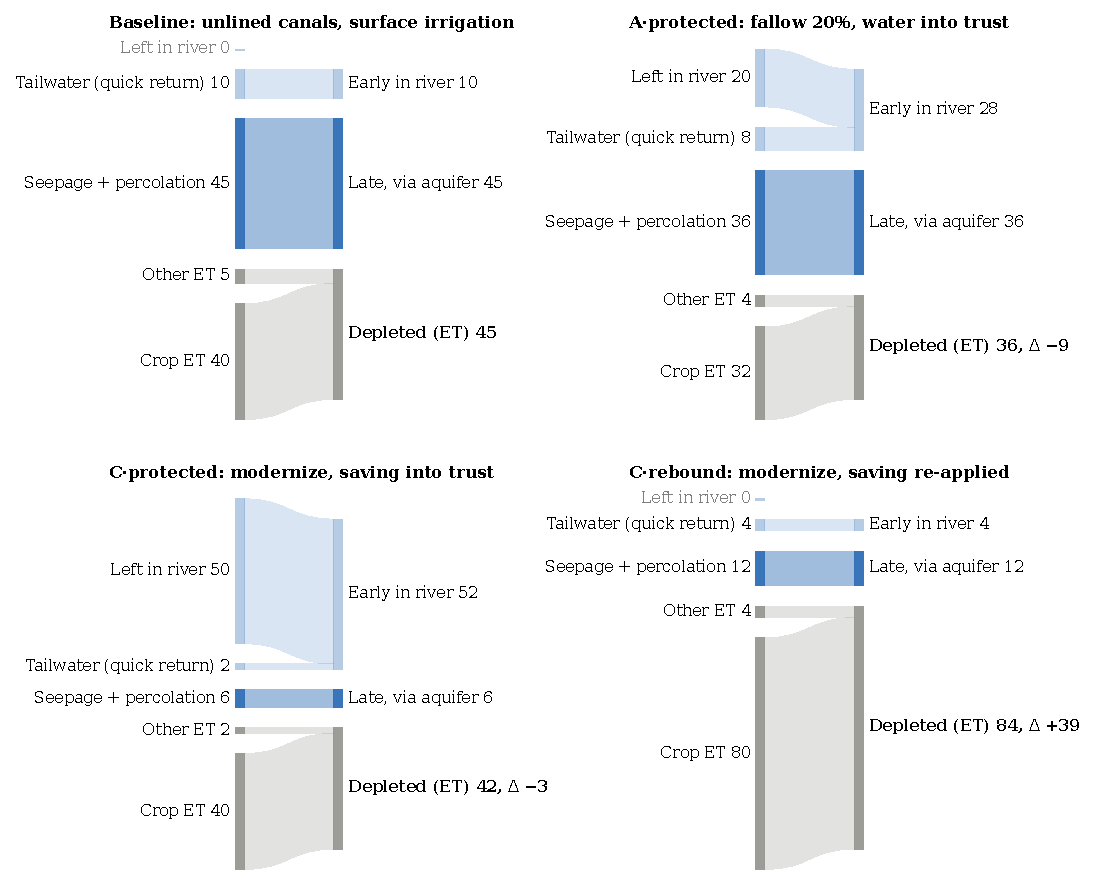
\includegraphics[width=\textwidth]{figures/sankey.pdf}
\caption{What managers measure (left of each panel) and what the basin receives (right), for the illustrative 100-unit district. \todo{Consider a version of this figure without symbols.}}\label{fig:sankey}
\end{figure}

% ===========================================================================
\section{What to report}\label{sec:report}
% ===========================================================================

\todo{A one-page checklist for funding applications and environmental review, matching the disclosure template in main.tex, Section 8.}

\begin{itemize}
  \item The reported saving, split into its wet and dry parts.
  \item The practice type (A to D) and where the freed water goes.
  \item The share of the reported saving that becomes basin water.
  \item The expected change in flow at named downstream points, early and late in the season.
  \item Whether the practice deepens a shortage at any point where flow already falls short of what is needed.
\end{itemize}

% ===========================================================================
\section{Using the Conserved Water Ledger}\label{sec:tool}
% ===========================================================================

\todo{Short guide to the interactive tool (repository yoderwsu/water-conservation-tool): what each control means, how to read each chart, and its main assumptions. This section can double as the tool's user guide.}

% ===========================================================================
\appendix
\section{Glossary: words and the symbols they stand for}\label{sec:glossary}
% ===========================================================================

This guide uses words only. Table~\ref{tab:glossary} links each term to the notation in the technical paper, for readers who want to move between the two.

\begin{table}[htbp]
\centering
\caption{Plain-language terms and the corresponding notation in the technical paper.}\label{tab:glossary}
\small
\begin{tabularx}{\textwidth}{@{}p{3.6cm}Lp{2.4cm}@{}}
\toprule
Term & Meaning & Technical paper \\
\midrule
Withdrawal & Water diverted or pumped by a use & $W$ \\
Consumed or lost water & Water that leaves the basin for good: plant use, evaporation, export, flow to a sink & Depletion $D$ \\
Beneficial consumption & Plant use or evaporation that delivers the intended service & $C_b$ \\
Non-beneficial consumption & Evaporation and plant use that deliver no service, such as soil evaporation and weeds & $C_n$ \\
Lost outflow & Water that leaves usable reach, such as flow to a saline sink or the ocean & $N$ \\
Return flow & Water that comes back to a usable river or aquifer & $R$ \\
Reported saving & Drop in withdrawal for the same service, before the freed water is used again & $F$ \\
Wet saving & Part of the reported saving that would have been consumed or lost & $F_{\mathrm{wet}}$ \\
Dry saving & Part of the reported saving that would have returned anyway & $F_{\mathrm{dry}}$ \\
Protected, rebound, transferred, banked shares & Shares of the freed water that go to each destination & $\lambda_s, \lambda_u, \lambda_t, \lambda_b$ \\
Change in basin consumption & Net change in water consumed or lost to the basin & $\Delta D$ \\
Basin share of the saving & Share of the reported saving that becomes water for the basin & Efficacy ratio $\phi$ \\
Flow needed & Flow required at a point and time, such as an instream target or downstream demands & $\underline{Q}_k(t)$ \\
Shortfall & Amount by which flow falls below the flow needed & $S_k(t)$ \\
\bottomrule
\end{tabularx}
\end{table}

\bibliographystyle{plainnat}
\bibliography{refs}

\end{document}
